% id: 0558
% book: RPM 중3-2 수학 · 05 대푯값과 산포도
% section: 유형 06 편차
% figure: crop:fig-0558.png
% answer: ③
% answer_source: 답지
% variant_level: 0 (원본 전사)
% 이 파일은 build.mjs 가 items.json 에서 만든다. 고칠 때는 items.json 을 고친다.
\smash{\raisebox{1.5mm}{\dmkichul{대표문제}}}
다음 표는 $\pt{A}$, $\pt{B}$, $\pt{C}$, $\pt{D}$, $\pt{E}$ 5명의 수학 점수에 대한 편차를 나타낸 것이다. 이 자료의 평균이 76점일 때, $\pt{E}$의 수학 점수는?
\par\smallskip\begin{center}\setlength{\dmfigw}{240.7pt}\ifdim\dmfigw>\linewidth\setlength{\dmfigw}{\linewidth}\fi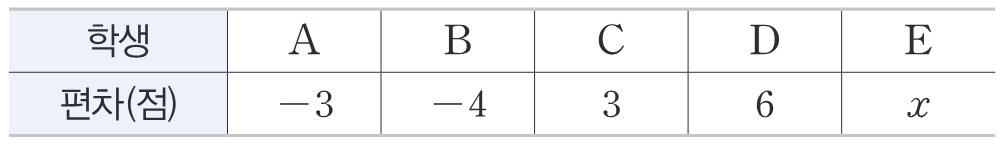
\includegraphics[width=\dmfigw]{figures/fig-0558.png}\end{center}
\dmchoicesauto{}{72점}{73점}{74점}{75점}{76점}
